\documentclass[12pt]{article}

%% Language and font encodings
\usepackage[english]{babel}
\usepackage[utf8x]{inputenc}
\usepackage[T1]{fontenc}

%% Sets page size and margins
\usepackage[a4paper,top=2cm,bottom=2cm,left=2cm,right=2cm,marginparwidth=1.75cm]{geometry}

%% Useful packages
%\usepackage{ams}
%\usepackage{amsmath}
\usepackage{graphicx}
\usepackage{tikz}
\usepackage{pgfplots}
\usepackage{hyperref}
%\usepackage[colorinlistoftodos]{todonotes}
%\usepackage[colorlinks=true, allcolors=blue]{hyperref}

% table options
\usepackage{multirow}
\usepackage{arydshln}

\setlength{\dashlinedash}{0.2pt}
\setlength{\dashlinegap}{4.5pt}
\setlength{\arrayrulewidth}{0.2pt}

% bibliography 
\usepackage{natbib}
\bibliographystyle{humannat}

\title{Using artificial intelligence to improve decision-making in conservation conflicts \\\medskip Annotated readings}
\author{Bach Adrian}

\begin{document}
\maketitle

%\newpage
\tableofcontents

\section*{Interesting sentences}
When  the  actions  of  one  party  clashes  with  the  objectives  of  another  party,  the  objectives of  one  might  be  expressed  at  the  expense  of  the  other,  causing  conservation  conflict \citep{duthie2018}.\\
Currently,  there  is  no  standard  way  to  measure  conservation  conflict  in  a  social-ecological  system  where  both the  natural  resource  (e.g.,  animals,  plants,  or  non-biological  resources)  and  the  people  (e.g.,  stakeholders,managers,  etc.)  are  modelled  in  a  single  system,  and  previous  modelling  approaches  have  not  meaningfully separated  agent  objectives  from  agent  actions. A  starting  point  to  developing  a  useful  metric of  conservation  conflict  is  to  quantify  the  deviation  of  an  individual’s  actions  from  their  objectives  (i.e.,  of actual  actions  from  desired  actions) \citep{duthie2018}.\\
GMSE  does  not  currently distinguish  female  and  male  individuals \citep{duthie2018}.\\
Conflict  might  persist  around  the  appropriate  target  population  size  rather  than  what actions  are  permitted  for  farmers;  currently,  this  potential  aspect  of  conflict  is  not  modelled,  but  future versions  of  GMSE  may  attempt  to  incorporate  such  additional  complexity  in  conflict  scenarios \citep{duthie2018} = Negotiations around manager's targets and policy.\\
Future  versions  of  GMSE  will  allow  users  to affect  one  another  directly  (representing,  e.g.,  different  groups  of  agents  lobbying  for  different  interests,among-user  conflict,  etc.) \citep{duthie2018}.\\
"No player can do better without the other player being worse off". Solutions with this property are called Pareto optimal \citep{COLYVAN20111246}. It is a solution from where the system cannot move without at least one player being worse off (includes both players being worse off).\\
If no player would unilaterally change his or her action from a solution without loosing personal outcome, it is a Nash equilibrium (supposes that the player knows what the opponent strategy is).\\
Herein lies
the real value of game theory: it provides a general and powerful
framework for analysing environmental decisions, one that
adopts a dynamical approach to decisions and naturally lends itself to an appreciation of the ongoing and far-reaching consequences of major environmental decisions. \citep{COLYVAN20111246}\\

Early  development  of  management  strategy  evaluation  (MSE)  models  originated  in  fisheries (Polacheck  et  al.,1999; Smith  et  al.,1999; Sainsbury  et  al.,2000) \citep{duthie2018}.\\

All models are wrong, but some are useful. George Box\\

Jeremy's talk (time series analyses in ConFooBio, budget optimisation and users compliance):
\begin{itemize}
    \item Assessed the quality of a strategy with the (actual, not estimated) population deviation from the manager's target.
    \item The managers' impartiality does not influence the user compliance, they do whatever they want in the limit of their budget.
    \item Engagement (involving users in the policy) increases compliance way faster and higher than enforcement (force then into doing something through pressuring their budget).
    \item  Genetic algorithm is a good candidate to model human thinking as it does not review every single possible strategies to select the best one, it selects the most fitted to its interests in a restrained population (along with discussion with Brad).
\end{itemize}
Moreover, the selection process through generations allows for stochasticity through mutation and crossing over. Hence the fittest strategy is not necessarily the optimal one, which could be interpreted as the fact that humans do not always chose the optimal option. \\

Holistic: characterized by the belief that the parts of something are intimately interconnected and explicable only by reference to the whole. (Google dictionary)

Median and average are means to reduce the information of a data set to a single value.
2D Linear regression reduces it to 2 values (slope and intercept).
Several algorithms for linear regression: least sum of deviation (robust to outliers), least sum of squared errors (more sensible to outliers because the deviation is squared), maximum likelihood (error distribution given the data set and the parameters), ...

\section*{Ideas}
Allow GMSE to build the world according to a GIS layer for landscape.\\
Include randomness into decision-making ? Already there, in the genetic algorithm: the decision is not optimal, it is just the best the agent could think of.\\
Use impact to assess the quality of a policy?\\
Use readings to justify the need of an adaptive model such as GMSE. Given which models have been used in previous studies.\\
How to justify the strength of the causality link between management actions and resource's response?\\
Try to formalize a ConFooBio case as a game.\\
\textbf{Lit review has to present a very clear path from a large question (something like: "how modelling can help settling efficient management strategies in conservation conflicts ?") to a more specific question that will be the one I will be treating during the PhD, backed up by former studies.}\\
Be strong on the definitions of \textbf{conservation}, \textbf{conflict}, \textbf{utility}, \textbf{game} in the theoretical sense, \dots\\
Emphasize on the fact that a sustainable conservation strategy is not to focus on nature only, but to find trade-offs between humans' interests and biodiversity.\\
\textbf{WHY SEEKING CONSERVATION ?}\\
Cognitive bias : anchor effect. We usually need a first guess to calibrate our judgement, but the utility associated with this guess strongly influences the way we estimate the alternative options' utility.\\
design a survey on how people perceive AI.\\
\textbf{I could use EVPI to assess the most impacting interaction to implement.} Would require a very precise question!\\
Be aware of a good trade of between over and under-fitting, or between too flexible and too rigid.

\subsection*{Brad meeting on 12th of October}
Lands close to public areas suffer from a higher problematic population, because resources reproduce faster in public areas. Plus, the other landowners scare theirs away. There might be a need to adapt policies to public areas proximity.\\
GMSE is implemented well enough because, following rules based on real cases observations, it succeeds in finding policies that equitably conserve the species and maintain users yield.
Even if it can not fit perfectly to all the possible situations (which is not its goal), the model can help to spot relevant aspects of the conflict that were neglected before.
It is meant to be compared to actual cases, highlighting important factors, and to provide help for decision-making, giving an idea of the long term consequences of a policy in an idealistic situation.\\
%GMSE is a decision helping tool, allowing a long term idea of the consequences of the policy. It is also useful to sort out which behaviour or which phenomenon that were not implemented in the model can make it deviate from the actual case, meaning they are worth paying attention at.
Comparing to real case studies to asses the robustness of the model would not be relevant because of the myriad of uncontrollable factors that can influence population dynamics, spatial distribution and users choices.
Plus, it's very costly.
But would be a good way to show the flexibility of GMSE, showing that it could provide a suitable strategy without the need for full knowledge of the possible sources of variation in decision-making or population dynamics.
Implementing random factor to simulate unexpected events, the fact that agents are not game theory experts, and can sometimes not choose the best option, would require an actual justification, why would it be interesting?
What question would it answer?
Note that the genetic algorithm already introduces stochasticity in the decision-making.\\
GMSE is predicted to be used by managers, or research scientists, but it could also be a way for "users" to understand why they are imposed quotas and interdiction.
Nonetheless, it would require a more friendly interface.\\
The 80 stakeholders simulation took ca 12 hours, also because the population was very large.
But it shows that the genetic algorithm could use parallelisation.\\
To show GMSE needs improvement, point at the situations where the four criteria of a successful strategy are not fulfilled. E.g : when the population is well managed but implying a broader income difference between the users. This could be a reason for the users (or the managers) to change the population target for example, should it be through negotiations.
Brad's idea: use a measure of conflict as a threshold to initiate interactions (e.g: negotiations).\\
Implementing a estimation-type-dependent population variation (estimated population and population target difference) threshold under which managers would rather not intervene at this time step, and see what happens.
Maybe allowing them to save some budget for next time step.
Good training on C. The increase in budget must be coherent with what the budget represents.
It could be a mix of money, time, energy, well-being.\\
Cognitive bias in negotiations: anchor effect.\\
ConSerVation / ConVerSation. When you turn the Versus over.\\
Dress a non-exhaustive list of the different models used in conservation management.

\section*{GMSE:  an  R  package  for generalised  management  strategy  evaluation - Duthie,  AB,  et al.  (2018).}

\textbf{Key words}: Conservation, conflicts, adaptive management, genetic algorithm, spatially explicit population dynamics, goal-oriented behaviour.\\

According to GMSE framework, a satisfying management strategy implies (not in order of importance):
\begin{itemize}
    \item Equitable spatial distribution of the resource on users lands.
    \item Focal species abundance stays close enough to the manager target.
    \item Users yield reaches a satisfactory percentage.
    \item Low differences between users yields.
\end{itemize}

Basic functioning of GMSE.
\begin{enumerate}
                \item A population of discrete resources (e.g.,a managed species) with individual traits (e.g., location, age) is modelled on a spatially-explicit landscape and can simulate resource birth, movement, interaction with the landscape, and death; the discrete nature of resources causes demographic stochasticity, and therefore uncertainty. %This sub-model is unique in not relying on other sub-models because ecological dynamics can be simulated in the absence of observation and management.
                \item Observation is modelled in one of four ways: resource counting on a subset of landscape cells (e.g., Nuno et al., 2013), marking and recapturing a fixed number of resources, and resource counting across the whole landscape either one linear transect or one rectangular block at a time (during which resources might move). Sampling error from all observation types generates a range of uncertainties that depend on monitoring effort.
                \item Managers analyse data collected from observations to estimate resource abundance, then compare this estimate with their predefined target abundance. Policy is developed by calling the genetic algorithm, which works within a manager constraints to find costs for user actions on the resource (e.g., culling, scaring, etc.) that minimise deviation from the target abundance, as informed by the predicted consequences of each action on resource abundance and user action histories.
                \item After a suitable policy is found, users perform actions that affect resources or landscape cells. Users respond to policy individually, each calling the genetic algorithm to find actions that maximise their own utilities (e.g., maximise resource use or landscape yield) within their imposed constraints. Once each user has found an adaptive strategy, user actions affect resources and landscape cells, feeding back into the resource sub-model.
\end{enumerate}
\begin{center}
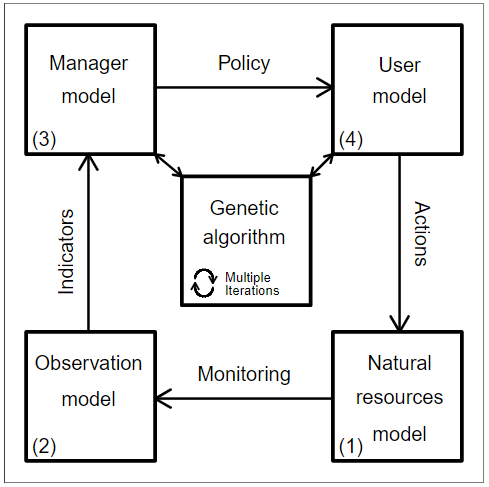
\includegraphics[scale=0.5]{GMSE-diagram.PNG}
\end{center}

Genetic algorithm: called each time a manager or a user has to make a decision. Generates a unique population of strategies (e.g. for a manager, allow such budget to such change in the cost of actions) with an associated fitness. The algorithm allow them to "\textbf{cross-over and mutate}" and re-evaluates their fitness. After burning some iterations, the decision is made when the fittest strategy fitness increase is below a chosen threshold.\\

SI1:  Each  run  of  the  genetic  algorithm  mimics  the evolution  by  natural  selection  of  a  population  of  potential  manager  or  user  strategies  over  multiple  iterations.\\
Deeper in the code for ACTION arrays, the  first  column Act identifies the  type  of  action  being  performed;  a  value  of  -2  defines  a  direct  action  to  a  resource  (e.g.,  culling  of  the resource),  and  a  value  of  -1  defines  direct  action  to  a  landscape  (e.g.,  increasing  yield).  Positive  values  are currently  only  meaningful  for Manager\_Actions,  where  a  value  of  1  defines  an  action  setting  a  uniform  cost of  users’  direct  actions  on  resources  (i.e.,  costs  where Act  =  -2 for User\_1\_Actions and User\_2\_Actions). \textbf{It's a key value to add interactions between agents, e.g. a value of X is a direct action on user1 specifically)}\\
\textbf{Adding a new type of stakeholder = a new layer in ACTION array}\\
The  fitness  of  each  layer  is evaluated  based  on  how  the  layer  is  predicted  to  affect  resources  or  landscape  output  to  which  the  agent  has assigned  some  utility. \\
\textbf{Cross-over}:  each individual  selects  a  partner,  then  exchanges  corresponding  array  elements  affecting  agent  actions  (columns 8-13)  with  their  partner  at  a  fixed  probability  of ga\_crossover.\\
\textbf{Mutation}:  For  each  array  element,  a  random  uniform  number u$\in$[0,1] is  sampled.  If u is greater than 1  -  (0.5  *  ga\_mutation),  then  the  value  of  the  array  element  is  increased  by  1.  If u is  less than 0.5  *  ga\_mutation,  then  the  value  of  the  array  element  is  decreased  by  1. Increase mutation if u is close to 1, decrease mutation if very close to 0, otherwise nothing. \\
\textbf{fitness}:  Individual fitness  is  defined  by  a  real  number  that  increases  with  the  degree  to  which  an  individual’s  actions  are  predicted  to  increase  entities  of  positive  utility  and  decrease  entities  of  negative  utility.\\
\textbf{Land utility}: When land\_ownership  =  FALSE(default,modelling  users  that  harvest  resources),Uures=−1 and Uuland=  0,  and  when land\_ownership  =  TRUE, Uures=  0 and Uuland=  100(modelling  farmers  trying  to  increase  crop  yield).

Genetic algorithm is well adapted to management strategies because it's a \textit{I know it when I see it} approach. No prior knowledge of the best solution, but ability to judge the quality of a proposition and, compare it to previous ones.\\

Geese example (scare or cull): Only the estimates of population size from the observation model are available to the manager, so policy change at any time step is driven primarily by the deviation of the currently estimated population size from the manager’s target and the actions of farmers in the previous time step. Hence, when the population size is estimated to be below (above) the manager’s target, the manager increases (decreases) the cost of culling and decreases (increases) the cost of scaring. Because the manager does not know in advance how farmers will react to policy change, they assume a proportional response in total actions with respect to a change in cost (e.g., doubling the cost of culling will decrease stakeholder culling by1/2). Farmers responding to policy are interested only in minimising waterfowl’s exploitation of their crops, so they will either cull or scare to remove the waterfowl from their land, depending on which option is more effective (i.e., cheaper).\\

\textbf{Further improvement for the genetic algorithm}: Future  versions  of  GMSE  might  improve upon  these  heuristics  to  generate  more  accurate  or  more  realistic  models  of  human  decision  making.  Such improvements  could  incorporate  additional  information  such  as  memory  of  actions  from  multiple  past  time steps,  or  a  continually  updated  estimate  for  how  actions  are  predicted  to  affect  resource  abundance  or  landscape output  in  a  simulation  (e.g.,  through  a  dynamic manager\_sense).  Alternatively,  future  improvements  could usefully  incorporate  knowledge  of  human  decision  making  collected  from  empirical  observation  of  human behaviour  during  conservation  conflicts.\\  

\textbf{\texttt{gmse\_apply}}: we  can  use  it  to  study  change  in  policy  availability. E.g.  what  happens when  scaring  is  suddenly  introduced  as  a  possible  policy  option. To see  how  manager  or  user  power  changes  over  time.  If  users’  budgets  increase  by  100 every  time  step,  with  the  manager’s  budget  remaining  the  same.  The  consequence  of  this  increasing  user budget  is  higher  rates  of  culling  and  decreased  population  size.\\
To avoid crashes, when an argument that changes the data structure is added, gmse\_apply builds a new set of agents and a new world at each call.\\

The aim of GMSE is not only conservation or maximising human activity income, but to reduce the conflict in a equitable way.\\

\textbf{SI6}: GMSE  might  be  used  to  assess  the  risk  of  extinction  in  a  managed  population, through repeated simulations varying in the frequency of managers intervenes. Possibility of extinction increases exponentially with this frequency.

\section{Models in ecology}

\subsection{Theory and models in Ecology: a different perspective. (Caswell, 1988)}
\textbf{Key words}: Theoretical approach, experimental approach, models, legitimacy, critique.\\

Fight the unjustified criticism towards mathematical models in ecology.
Mathematical models allow the exploration of the possible patterns, which suggests "new ways of looking at problems".
Theory in biology aims at exploring the range of possible patterns in order to identify the systems boundaries ("this can happen, this cannot").
One cannot expect theory to be infallible, as any knowledge accessible to us, including experimental one, it is \textbf{conjectural}. 
Experimental approach is compulsory when testing if a theory actually applies in nature, but it cannot answer questions on the theory itself while modelling approach can. For example, when searching for the least assumptions to predict a given phenomenon.

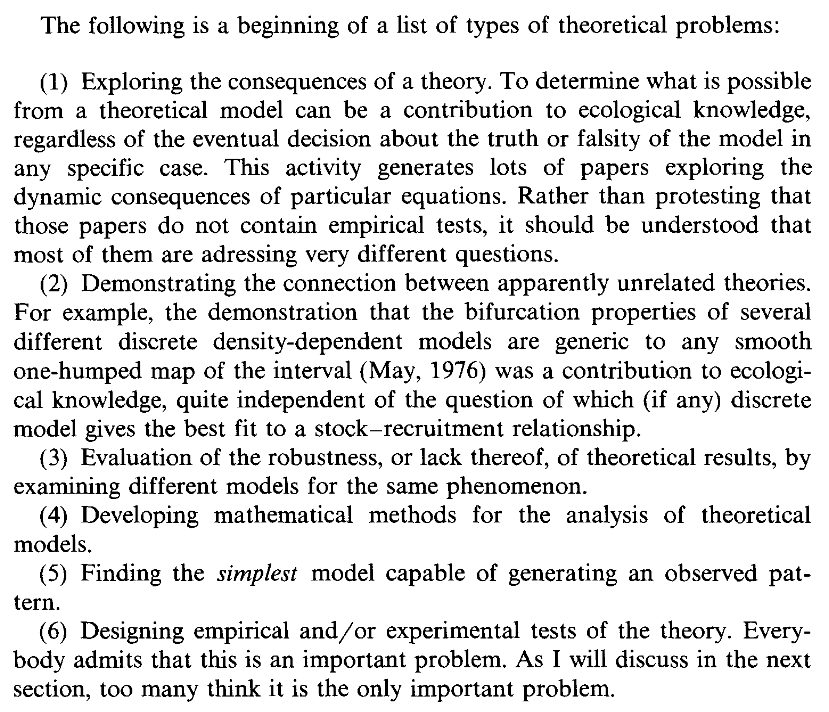
\includegraphics[scale=0.5]{theoreticalProblems1988.png}\\
\textbf{Which one is GMSE?} Brad: it could pretty much be all of them. In general, it would be a (4), in the sense that it uses novel computational methods to model conflicts management, but it could be used for all the other possibilities. Basic use of GMSE is probably (1), it explores possible outcomes using the current situation as initial conditions. We could also argue that GMSE links decision-making theory to population dynamics, which would fit in (2).

Testing is not the only thing to do with theories. First, they need to be developed, and preventing people to develop theories without any backing-up data would result in slowing the discipline.\\
Refute a theory is not abandoning it, it is an encouragement for improvement.\\
"Does the model include such important factor (related to my field of study) ?". Irrelevant most of the time. Just as most experimental set-ups assessing one to two factors in relation to an other, the theoretical approach cannot take all the factors into account, and must also focus on the variables relevant to its research question.\\
\textbf{"\textit{models are to theoretical problems as experiments are to empirical problems.}"}

\subsection{Individual-based  modelling  and  ecological  theory: synthesis  of  a  workshop (Grimm 1999)}
\textbf{Key words: individual-based modelling, ecology, conservation, review, complexity.}

3 main arguments against the use of IBMs in Ecology: " complex  models  are  hard  to develop,   hard to   communicate,   and   hard   to understand."\\
The only way to communicate models is through verbal and mathematics description, but the core of the model is the code, which is incommunicable by definition. It is where all the errors and bugs can dwell, thus falsifying the information taken out of it. No one has the time to implement the model him/herself based on the verbal description. (ndlr - same for experiments by the way! It's time costly to redo an experiment.) Beware of putting more effort in the coding than the the analysis, it could lead to a "WhatYouWantIsWhatYouGet" fallacy. Models has to be as simple as possible! Unnecessary complexity, although being an interesting challenge, would just result in the model being harder to communicate and analyse, thus reducing its scientific value.\\
Models can definitely help pointing at stuff that needs to be studied in order to understand a mechanism. It's even better to use \textbf{a suite of different model implementations} to prove that the way you code the model does not change the conclusion.

\subsection{NEW HORIZONS FOR MANAGING THE ENVIRONMENT: A REVIEW OF COUPLED SOCIAL-ECOLOGICAL SYSTEMS MODELING (Schlüter, 2012)}

\paragraph{Chapter 3.2.3.} "One of the problems with many traditional decision-making tools in natural resource management is that their outcomes depend on humans behaving in a defined and predicable manner."
"Unexpected responses of humans to management interventions have been identified as one of the key sources of uncertainty in fisheries management (Fulton et al. [2011]) and wildlife conservation (Keane et al. [2008]). Due to unforeseen behavioral responses of users or consumers or their non  compliance with rules, a measure taken to enhance ecosystem services does not necessarily lead to the expected outcome or may even worsen the situation."\\
MSE "is also being introduced in a wildlife-management context (Chee and Wintle [2010]) and in catchment management (Turneret al. [2003])."


\section{Management strategy in conservation conflicts}

\subsection{Conservation and the Myth of Consensus (Peterson, 2005)}
\textbf{keywords}: Argument-based, Consensus-based, Constructionist, Sustainable development, Democracy.\\

From a constructionist perspective, nothing is "real" for humans until they reach a consensus about it.
Any idea stays "rhetorical" unless a community makes it "reality" by commonly agreeing on its meaning.
Consensus is a unconditional step in the realisation of any idea.
But very often, different consensus are reached in different communities, which -according to constructionist thinking- leads to the emergence of different realities.\\
Reaching a consensus on the fact that conservation can go alongside with economical growth is possible, but would require to ignore research work and personal experience that prove the contrary. In this sense, the very notion of consensus of conservation in our growth-oriented societies faces a wall.\\
Management by consensus is risky because tying to meet every stakeholders expectations need agreement processes that can slow -sometimes eliminate- the impetus for a change. Moreover, such question usually arise within organised communities where some instance has the power to orientate the consensus in a way that does not threaten the current hierarchical positions.\\
Commonly accepted definition of sustainable development : "A development that meets the needs of the present without compromising the ability of future generations to meet their own needs".
A definition based on which every "community" built its own reality, resulting in very different points of vue.\\
"The emphasis on win-win outcomes in consensus-based models for environmental decision making is problematic in part because we achieve the illusion of objectivity and universal reason only by bracketing or masking conflicts among participating groups and individuals. We thus treat as truth that which could just as easily be understood as hegemony. As Mouffe (2000) contends, the illusion of consensus is fatal to democracy because a healthy democratic process requires recognition of differing interests and the recognition that open conflict about differing interests is legitimate."
To avoid conflict and to secure their position, "dominant elites generally prefer consensus-based approaches over those based on argumentation". Interesting for GMSE.
Ivie (2004) specifies that, “democratic dissent in a period of war or crisis is as alarming to the purveyors of prevailing opinion as it is critical to a nation’s political welfare.”
Consensus strengthen current political instances and their globalised, growth-oriented view of the world, thus produces nothing remotely sustainable.\\
"The hypothetico-deductive scientific method suggests reality only by methodically eliminating alternatives (Murphy \& Noon 1991), not by proving truths." Thus, it cannot provide any answer for a policy question.\\
\textbf{"Why focus our efforts on on achieving the improbable and possibly unwanted goals
of monism in science and government, when an emphasis  on  negotiation  (de  Graaf  et  al.  1996) within democratic processes (Mouffe 2000) can explicate the implicit value judgments required for conservation to be successful, and simultaneously empower citizens to participate in the application of science to democracy? Within this argument-based model, environmental decision making reflects deliberation, debate, and conflict about both direct and indirect scientific observations of the physical world."}\\
"Consensus-based approaches to environmental  policy  are  necessary  but  insufficient  to  ensure the best decisions. An emphasis on argument legitimises and facilitates change, whereas an emphasis on consensus further legitimises continuity or stability."

\subsection{Uncertainty and adaptive management for biodiversity conservation (Keith et al., 2011)}

(Literature review)\\
\textbf{Key words}: Management quality, comparative studies, role of modelling, estimated value of perfect info.\\

Comparative study of different strategies on the field : " Its key elements include explicit
definition of management goals, development of plausible alternative management strategies to achieve those goals, implementation of two or more strategies in a comparative experimental
framework to spread risks of management failure and improve
understanding of system responses to management, monitoring
to evaluate the relative merits and limitations of alternate strategies, and iterative modification of management strategies to improve management outcomes (Lindenmayer and Burgman, 2005)"\\
Since the response to a policy is lost into other responses from a myriad of uncontrollable external factors, monitoring the system's response to a policy over time seems not to be a good way to test and improve the policy. Also very costly! And the information gathered are most of the time estimations, that can mislead management if too far from real info. \textbf{Estimated Value of Perfect Information} can help targeting the most efficient commitment to monitoring and its scale of precision.\\
"Models are imprecise representations of complex ecological
systems, and at best can typically only predict directions of change
in response to management policies. Yet models can be extremely
useful tools that help clarify management problems and identify
important knowledge gaps that question faith in model predictions."\\
Some people implemented a way to compare different policy models in terms of learning and conservation efficiency.\\
Scientists "sometimes use policy
demands to pursue discovery goals that may never be applied to
decision making by testing their predictions. Managers often wilfully ignore scientific uncertainty to avoid complicating their message to stakeholders, and use it (or the pretence of certainty) later
when policies fail in attempts to shift responsibility for failed policy implementation to the scientific community".

\subsection{Which uncertainty? Using expert elicitation and expected value of information to design an adaptive program (Runge 2011)}
\textbf{Key words}: Expected Value of Information, Expert Elicitation, Decision-making, Conservation, Adaptive Management, Workshop.\\

\textbf{"Natural resource management is plagued with uncertainty of many kinds, but not all uncertainties are equally important to resolve."}\\
"The promise of adaptive management is that learning in the short-term will
improve management in the long-term."\\
Using the Expected Value of Perfect Information (EVPI) to anticipate the impact of the resolution of an uncertainty on the efficiency, or informativity, of a management strategy.\\
"several taxonomies of uncertainty (Morgan and Henrion, 1990; Regan et al.,2002)."\\
"by addressing epistemic uncertainty in the short term, we can improve management outcomes in the long-term. "\\
The utility for GMSE would be the level of conflict? The focal species population? Users income? The answer is that the "utility scale has to be relevant to the decision maker".\\
"The challenge with these value of information methods is that
they require articulation of a set of models (hypotheses), a prior
belief about the credibility of those models, and predictions of
the outcomes under each model and action combination."\\
For prior knowledge, we can refer to expert elicitation using one of the many existing "Delphi" methods.\\

"The management problem was framed as a multi-criteria decision analysis under uncertainty: what management strategy should
be undertaken at NNWR to benefit the EMP of whooping cranes, as
expressed through four objectives, in the face of uncertainty about
what is causing reproductive failure? This analysis involves manag
ing tradeoffs among several objectives, as well as examining the im
pact of several specific hypotheses for reproductive failure. To
develop this framework, we needed to specify the objectives, artic
ulate the hypotheses for reproductive failure, develop potential
management strategies, and predict the outcomes of each strategy
on each objective under the alternative hypotheses."
Identify objectives, measures that can be associated with it, weight their relative importance, develop hypotheses on the reason why, attribute points for the relevance of each hypothesis to select a panel, and finally develop a management strategy to treat each hypothesis. Make predictions on the response of the objectives variables over a certain amount of time for each strategy under each hypothesis.\\


\begin{center}
    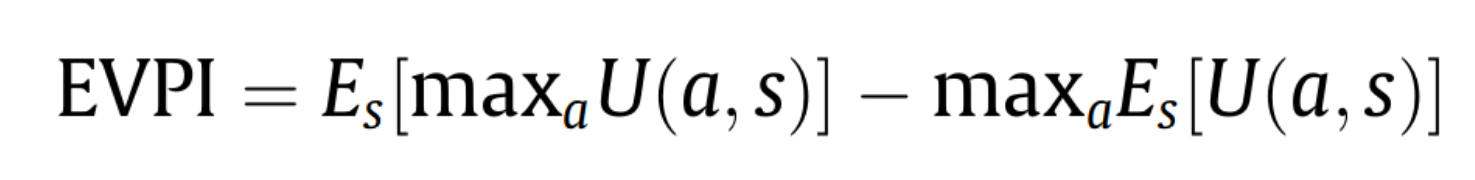
\includegraphics[scale=0.25]{EVPI-formula.png}
\end{center}
EVPI is the utility gain associated to the fact of knowing \textit{a priori} the best option. The first term is the utility of action a having the info about the best thing to do if the system behave a certain way \textit{s}. The second term is the utility of the same action without having prior knowledge of the best thing to do.
A positive EVPI traduces a information worth than investment. But only if "it is possible to reduce the uncertainty through monitoring, and whether the short-term costs of acquiring the information are off-set by the long-term benefits of the information".

\subsection{A critical assessment of adaptive ecosystem management in a large savanna protected area in South Africa (Wilgen, 2011)}
\textbf{Keywords}: National park conservation, Strategy building, Consensus on thresholds, multi-stakeholder conflict, feedback, protected area.\\

Interesting to-do-list for planning an adaptive management strategy. can be useful for GMSE?

"The goals of protected areas usually include the maintenance of their component species, communities,
landscapes and ecological processes. [\dots] This approach integrates research, planning, management and monitoring
in repeated cycles of learning about how to better define and
achieve objectives." Users in the sense of MSE, are not taken into account in the cycle.\\
Conservation motivations: preserve local habitats, avoid threat on local species by invasive alien species, control animal population, maintain the existing interactions. Different purpose, mainly ecology and tourism.\\
First, all the stakeholders talk through a list of objectives associated with a priority. Then agreeing on lower and upper thresholds to give any objective a range of satisfaction.\\
Active adaptive policy: implementing rapidly policies in order to acquire information on the outcomes, both expected and unexpected.\\
"In complex socilogical-ecological systems, the achievement of desired outcomes through management intervention cannot be guaranteed, and, in addition, the outcomes may be replaced with
different ones that appear more desirable as understanding increases."\\
Example of difficulty of reaching a consensus: "A decade ago, conservation authorities and the government
were unable, in the face of conflicting evidence, interpretations
and opinions, to formulate an agreed policy on elephant management."\\
"Success may be complicated by the
fact that ecosystems are often slow to respond to management
interventions, or that the interventions could have unexpected
consequences."
\begin{center}
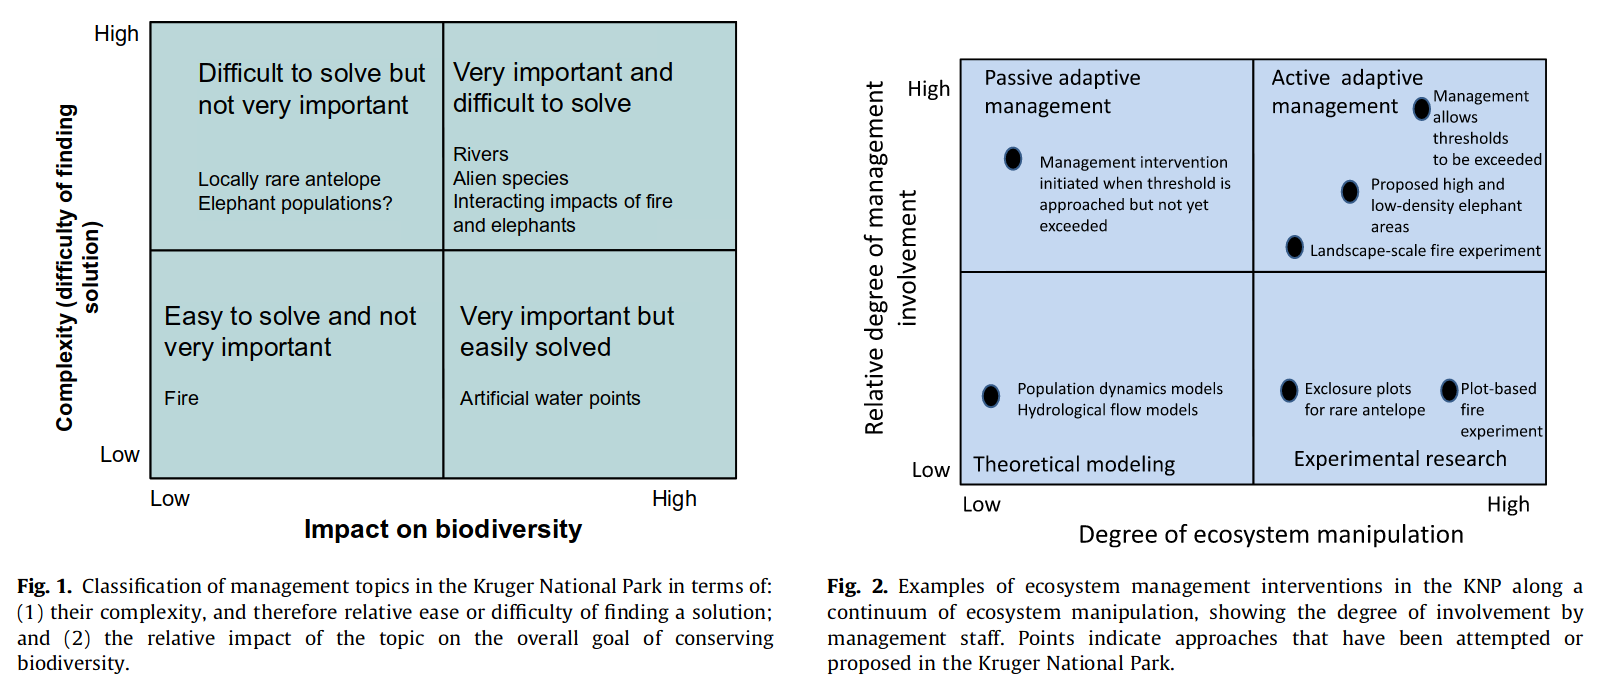
\includegraphics[scale=0.3]{managementClassification.png}
\end{center}
Management based on thresholds has proven to be quite difficult in terms of monitoring and accuracy.
Too much time spent on revising thresholds and changing monitoring methods.

\subsection{State-and-transition modelling for Adaptive Management of native woodlands (Rumpff, 2011)}
\textbf{Key words:} Landscape management, state and transition model, Bayesian network, expert elicitation.

"Adaptive Management is a ‘learning by doing’
approach that acknowledges management action must proceed
in the face of uncertainty, but facilitates iterative updating of
knowledge and management strategies (
Walters, 1986; Ringold
et al., 1996
). In this way, Adaptive Management ensures that future
management decisions are socially, economically, and scientifically
defensible."\\
"some of the problems
[preventing AM to be implemented], such as complexity of natural systems and uncertainty and
paucity of appropriate data about management effectiveness, are
the very factors that recommend Adaptive Management and its
promise of transparency and defensibility in management."\\
Most existing STM are said to "fail to meet three key requirements of a working model
for Adaptive Management: (1) quantitative predictive capability;
(2) representation of uncertainty in states and transitions; and
(3) amenability to updating as new knowledge accumulates."\\
"Quantifying system response allows us to make predictions about
the relative efficacy of management options and to identify and explore the ‘critical uncertainties’ that most impact on our ability to
accurately predict responses to management and, therefore,
choose the best course of action or the best investment strategy."\\
Everyone involved in conservation conflicts uses models all the time, but they are verbal (e.g. allowing geese-hunting will increase farmers income, planting these trees here will create habitat for birds and prevent weed development). When it comes to formalise them into something one can use for simulations (in order to predict systems response, identify uncertainties, or help decision-making), confidence in the model drops. Thus, it is believe to be something deeply scientific and invaluable in wildlife management.\\
The model complexity must be consistent with stakeholders expectations, and conservation goals.\\
"Transition $=$ A change in state, caused by the crossing of a
threshold value for one or more of the state
variables". Thresholds, states, variables, and transitions have been determined with several workshop with ecologists and natural resources managers.\\
All the states are not linked with transitions. A derived landscape can not shift to a reference state without going through the simple state. How do they justify it?\\
Differentiate biotic and abiotic factors that can be controlled by management actions (process) and the ones that management can not act on (independent).\\
They deal with uncertainty proposing to tweak thresholds, transitions, and states to compare results. I am not very satisfied with it.\\
Bayesian framework: simulate the transition probability given such and such management actions assuming prior knowledge on the likelihood of transitions under these particular management strategies; than monitoring and assessing actual transition probability; finally correct the model with actual prior knowledge on the likelihood. That way could spot which strategy was best and worse estimated.  way of \textbf{learning} for the Bayes Net.

\subsection{Management strategy evaluation: a powerful tool for conservation? (Bunnefeld, 2011)}
\textbf{Key words}: MSE framework, management conflicts, multi-model approach, conservation.\\

"The management of natural resources is a complex process driven by interactions between the dynamics of the natural system, the decision-making and behavior of stakeholders, and uncertainty at various levels of the management process and the natural system. Traditional forms of natural resource management (e.g. fixed harvest quotas) do not respond to system dynamics and uncertainty, and so are prone to failure. Realization of the importance of learning about the dynamics of the system led to adaptive management, in which monitoring of the system allows updating of managers’ models of system dynamics, which then produces alterations in the harvest in an iterative process."\\
"A key feature of the MSE approach is that an optimal strategy or solution is not pursued, but instead policies are sought that are feasible, robust to uncertainty, and which provide adequate management performance with respect to multiple criteria".\\
"MSEs can evaluate which data and how much of it should be collected and how often monitoring should be carried out to improve management performance."\\
Uncertainty occurs in each of the sub-models population dynamics, population estimation, institutional inertia and users compliance. Implementing them is also a way to quantify their relative importance.\\
"Management often works against the short-term economic interests of those who depend upon resources by decreasing the harvest or closing areas to protect its natural resources."\\
"[\dots] models on the line fishery of the Great Barrier Reef include how individual fishers [\dots] communicate
information amongst each other." (with references!)\\
GMSE "has been criticized for: (i) having a longer development time (and thus increased costs) than traditional methods such as reference-based off-take rules; (ii) an upfront MSE can provide an overly rigid framework without room for decision-makers to change management in an adaptive way; and (iii) poor data inputs (e.g., gaps in monitoring or extremely low estimates of uncertainty) affect the performance of MSE, which needs to be recognized and explored within the MSE process." Incapacity to monitor the focal species can also be a highly problematic factor for the implementation of a MSE.

\subsection{Conservation in a Wicked Complex World; Challenges and Solutions (Game et al, 2013)}
\textbf{Keywords:} complexity, wicked problems, inspirations from external fields, adaptive management critique.

"the characteristics of “complex systems”: numerous interacting elements lacking any central control, non-linear interactions between elements,constant change which is seldom reversible, and no clearly defined boundaries to the system (Rosser Jr 2001;Johnson 2007; Mitchell 2009)". In such wicked problem, it is very difficult, no to say impossible to isolate a feature from the other, as all characteristics are densely interconnected.\\
"There is no “right” solution to wicked problems in complex systems, only trade-offs that appear more or less favourable depending on your perspective.This ambiguity also means that there is rarely any need to declare conservation actions a failure".\\
Discussion about the relevance of AM in conservation.
"Less frequently acknowledged is that AM is, at least in part, appealing because it reduces cognitive effort and resources invested in planning; changing the maxim “Ready, Aim,Fire” to “Ready, Fire, Aim” (Patton 2011) though per-haps “Ready, Fire, Aim, Fire” is more suitable." 
Change of strategies are rare in AM, because assessing the adequacy of a strategy is still very challenging.
Another tricky problem is that implementing any decision will lead to a change in the system, thus learning from it can be misleading because the condition between the situations has already changed.
All that could mean that AM is relevant only in simple, small-scale problems.\\
Authors recommand to use multiple-scenari approach.\\
"Although conservationists routinely bemoan the lack of funds for their activities (McCarthyet  al. 2012), there is little evidence that bigger budgets make conservation easier or more effective."


\subsection{Conflicts in conservation: navigating towards solutions. (Redpath et al., 2015)}
\textbf{Key words:}\\

\subsubsection{Phylosophy, conflict and conservation (Alan Holand)}
Alan Holand emphasize in the second chapter that it is relevant to assess the impact of the policy (deviation from what would have happened if doing nothing).\\
Being aware of the consequences of a policy, because it can result in undesirable after effects (e.g. conservation of a certain gorilla species led it to be more vulnerable to human vectored diseases).\\
Questioning the statement that "more [biodiversity] is better", with a parallel with the tragedy of the commons.\\
About "commitment to nature", "conservation interest": "a highly complex and even puzzling concept". Examples of divergences: focus on individuals or on 'wholes' (populations, species, ecosystems, \dots), degree of sentience of non-human living beings (\textbf{Sentience is the ability to feel, perceive, or experience subjectively.}(Linguee definition)), the tolerance to the intrusion of 'non-indigenous' species in a ecosystem.\\
Environmental philosophers: Katz (1987), Elliot (1992), McShane (2007).\\
The 'conservation interest' should not be related to any individual interest of the conservationist (e.g. I like hiking/climbing/diving like any other researcher, so I want to conserve mountains/seas/oceans to keep on enjoying it in the future) but to a highly intrinsic value of nature regardless of how the conservationist sees it.
Plus, human interest and well-being is currently contingent with the welfare of the environment.
Conservationists often behave (probably not being aware of it) as the voice of nature, standing for its interests. But 'nature's interests' does not really make sense, [ndlr] because \textbf{as far as we can tell, except limiting its increase of entropy, an ecosystem is not a goal-oriented entity, neither has any affection for the individuals that compose it}.\\
Stoicism critique Mill 1874.\\
"The 'conservation interest' is just an important aspect of 'human interest' in general" in the sense that our survival depends on the fragile balance of ecosystems.\\
"[\dots] ideals and values are precisely the kind of things that do not normally allow negotiations or compromises."

\subsection{Goose management in Scotland: An overview (Bainbridge, 2017)}
\textbf{Keywords:} adaptive management, conflict, geese conservation, SNH, politics, deterministic population dynamics modelling.\\

Geese endangered status (recognised during the 1940's) was caused by "a combination of
hunting for food and sport, systematic persecution and the
disruption of the Second World War".\\
Protection measures were really efficient as, in the 1980's, all geese species population numbers increased significantly.
But this rise in population started a conflicts with farmers, as geese were grazing their crops.
Especially for farmers owning culture in Special Protection Areas required by the European Bird Collective.
The first arrangements between the state and these farmers concerning geese control were made in the early 1990's, in the form of payments from government for farmers to allow undisturbed grazing on certain areas, and scare them away in others areas.\\
Yet, some populations are still increasing nowadays, and farmers started to consider the financial compensation too low for the damages caused.
Scottish government refused to increase them for financial reasons.
Farmers then started to control the population by means unapproved by the government.
Time had come to implement adaptive management of this conflict.\\	
"In the absence of detailed population data, simple
deterministic models were developed." Sometimes, the shooting target was beyond the capacities of local communities.\\
"To summarise, the current position of goose management in Scotland is that there are a limited number of
winter schemes based on payments to allow feeding of
geese on agricultural land. There is a limited shooting
associated with these schemes (Islay only), and a general
trend to decreasing levels of funding; with a resulting
increase in farmer dissatisfaction and political activity."

\subsection{Time series analysis reveals synchrony and asynchrony between conflict management effort and increasing large grazing bird populations in northern Europe (Cusack, 2017)}
\textbf{Keywords: time series, management, large grazing birds, synchronicity analysis, users compliance.}

Synchronicity analysis on population, scaring counts, killing counts, and monetary compensations time series. Comparing the number of time steps where the time series were changing in the same direction, and compare it to a random distribution of the time steps.\\
Time series were sometimes synchronous and sometimes not. "inconsistent patterns of synchro- or asynchronicity".\\
"perceived randomness and inconsistent changes in management effort relative to wildlife impacts
in the short and long terms have been shown to influence the
level of trust stakeholders place on the decision-making process (Young et al., 2016), as well as their overall responsiveness to policy change (Olson et al., 2015)".\\
Encouraging managers to wait for proper information to act, so they can be synchroneous with changes in the system.

\subsection{Social conflicts increase the risk of natural resource mismanagement (Cusack, in review, 2018)}
\textbf{Key words}: management conflicts, lobbying, users compliance, illegal harvesting, GMSE.\\

"We   find   that   in   the   absence   of   disagreement   between   manager,   user   and conservation  objectives,  natural  resources  are  managed  effectively  regardless  of manager   impartiality   and   user   compliance   levels." Meaning all the stakeholders have the same population target? Budget?\\
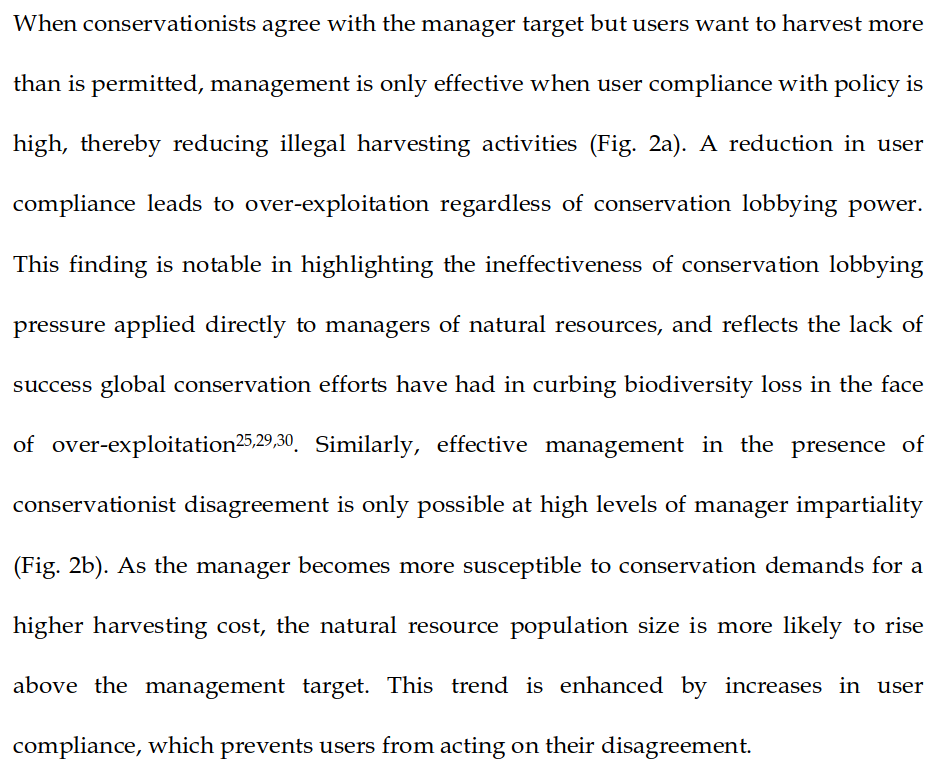
\includegraphics[scale=0.5]{cusack-results.png}\\
"[\dots] when  users  and  conservationists  show  a  symmetrical  disagreement  with  the manager’s  target,  the  influence  of  illegal  harvesting  on  management  outcome  is much stronger than  that of conservation lobbying [because] user actions  have  a  direct  effect  on  the  resource,  whereas  lobbying  targets  policy-setting by  the  manager,  which  does  not  directly  affect  the  natural  resource  population.  In other words, users have the “final say” on what harvest will be implemented [\dots]". Increasing users compliance has a greater effect on policy's efficiency than any other increase in the stakeholders characteristics.\\
"the impact of conservation lobbying is constrained by the  manager’s budget"?\\
"User compliance reflects how effective the manager is at preventing illegal harvesting by the user. impartiality represents how susceptible the manager is to lobbying by conservationists for a change in policy."\\
Probability  surfaces  represent  predicted values  from  a  Poisson  generalised  additive  model  with  a  smooth  tensor  product  representing  the interaction between manager impartiality and user compliance"???
In this paper, conservation lobbyist are supposed to aim at a the stated conservation population target because they are species-driven only, but managers and users are likely to aim at a lower target.
"Lobbying  can  be  broadly  defined  as  any  strategy  that  seeks  to  influence  policy  to benefit   a   specific   interest."
Lobbying intensity increases exponentially as the focal population approaches zero, and non-existent when it is above the conservation target. Is that consistent?\\
On the other hand, illegal harvesting intensity increases exponentially as focal population approaches \textit{K}, and is non-existent if users target is above manager target.
"The  second  would  seek  to  obtain  agreement  amongst different parties on the management target prior to actions being carried out." Back to consensus?\\
GMSE = "stochastic growth of the population"?\\
"Management effectiveness was assessed as the mean resource population size at time step 10 across iterations."

\paragraph{SI.} A major feature of MSE is to take into account uncertainty in all the key parts of conflict management: resource stochasticity, monitoring errors, (ndlr) and unoptimal decision-making. Jeremy tried to fill the gap of disagreement on manager's population target.\\
J emitted the idea that conservation lobbyists could influence the system by buying and protecting lands.\\
"management  target  can  be  achieved 
only 
for 
a  subset
of  all 
manager and user budget 
combinati
ons". Cf the 3D plot of J's seminar.\\
"To  counter  illegal  harvesting,  a  manager  may  seek  to  increase  user  compliance,  either 
through  enforcement  or  user  engagement."\\

\section{Game theory}

\subsection{Game Theory, Analysis of Conflict (Myerson,1997)}

\textbf{Key words}: games, utility, decision-making, cooperation, Nash equilibrium.\\

"\textit{Game theory can be defined as the study of mathematical models of conflict and cooperation between intelligent rational decision makers [which choices] affect one another welfare}."\\
Origins in WWII, to help understanding the issue of the nuclear cold war.\\
Games are simplified vision of actual conflicts, the actual complexity being unreachable to us. But such complexity would prevent us from understanding the fundamental issues of conflict and cooperation. As any other scientific work, game models deliberately omit less relevant details of actual situation to allow the study of particular phenomenon in the scope of a particular question.\\
Players act in order to maximise the expected value of its outcome $=$ \textit{utility}. Utility is not necessarily quantified as monetary pay-off, it can be time, effort saved, well-being, happiness, and even a mix of them.\\
Players are supposed to follow the expected utility maximising theorem. This theorem is consistent with the innumerable observations of evolutionary selection in biological system, doing whatever they can to survive and/or reproduce. It can go further in terms of entropy/order, all living being tends to consume order to slow the process of entropy increasing on their body (order being the expected utility to maximise).\\
The author refers to \textit{intelligent} as players that has knowledge of the game theory framework, and is able to reach the same inferences as a game theorist. It is a questionable assumption but consistent with the fact that humans are able to learn from mistakes. (?)\\
\textit{Bayesian decision theory.} Two models for utility function: probability model (objectives unknown) and state-variable model (subjective unknowns). Objective unknowns $=$ you know the outcome possibilities and their probabilities (e.g. lotteries). Subjective unknowns $=$ you do not know the probabilities (e.g. horse races).
A decision making model can be descriptive (show why a decision was the best for a player), or prescriptive (this is what you should do in this situation according to the model).\\
Several cases in which expected utility maximising is usually not respected.

\subsubsection{Models}

A model of too simple structure may miss key aspects of understanding, but a too complicated one can obscure fundamental issues.

\subsection{The conservation game (Colyvan et al., 2011)}

\textbf{Key words}: game theory, conservation conflicts, cooperation, top-down regulation, adaptive management.\\

Management strategy usually focuses on a single outcome, assuming a consensus on its utility among the stakeholders. In the context of conflict, such an approach is unproductive. It can be symptomatic of a certain partiality in conservation. Sustainable solution need to take all stakeholders interests into account (nature itself being also eligible as a stakeholder). Game theory framework is a better approach as it is designed to find each stakeholders actions that can lead to the best outcome for everyone.\\ 
Plus "game-theoretic perspective provides insights about: the strategies different stakeholders will likely adopt given their objectives when consensus, compromise, or cooperation are feasible; what types of cooperation best reflect stakeholder interests and achieve their objectives; which stakeholders are likely to form coalitions; the range of possible outcomes under non-cooperative and cooperative decision-making dynamics; and, whether an optimal or satisfactory solution for all stakeholders can be reached simultaneously".\\

Four main game theory examples (numbers represent gains) :
\begin{table}[ht]
    \centering
    \sffamily
    \begin{tabular}{l|r|c|c}
        \multicolumn{2}{l}{\multirow{2}{*}{}}    & \multicolumn{2}{c}{P1} \\ %\cline{3-4} 
        \multicolumn{2}{l}{}                     &      C     &     D      \\ \cline{3-4}  %\hline
        \multicolumn{1}{r}{\multirow{2}{*}{P2}} & C &     \textbf{2,2}      &      1,1     \\ \cline{2-4} 
        \multicolumn{1}{r}{}                  & D &     1,1      &     0,0      \\
    \end{tabular}
    \caption{\textit{Simple} game $=$ No costs for actions. E.g : two bordering countries cooperate for the management of a species at no cost. Both countries choosing to conserve is the highest personal gain both players can get. If one of the countries chose not to participate, personal gain is lower for both, which makes [C,C] Pareto optimal. There is no way that a player can be better off than the other by moving from [C,C], for any of the opponent strategies, the best option is always cooperation; making it also a \textbf{Nash equilibrium}.}
    \label{tab:sigam}
\end{table}
\begin{table}[ht]
    \centering
    \sffamily
    \begin{tabular}{l|r|c|c}
        \multicolumn{2}{l}{\multirow{2}{*}{}}    & \multicolumn{2}{c}{P1} \\ %\cline{3-4} 
        \multicolumn{2}{l}{}                     &      C     &     D      \\ \cline{3-4}  %\hline
        \multicolumn{1}{r}{\multirow{2}{*}{P2}} & C &     1,1      &      \textbf{1,2}     \\ \cline{2-4} 
        \multicolumn{1}{r}{}                  & D &     \textbf{2,1}      &     0,0      \\
    \end{tabular}
    \caption{\textit{Chicken} game $=$ action have a cost. E.g : two bordering countries face the problem of the management of a shared species implying costs (-1 in gain). Hence, if a party conserves and the other defects, the later enjoys some of the benefits from conservation without paying its cost, but the management is \textbf{as} efficient. Here, the system can always find a situation to move in so at least one party is better off, meaning there is no Pareto optimal situation. Knowing the other party strategy, the best outcome for a country would be [D,C], and if the situation stayed the same this country would have no reason to move away from its position. Since each party would have the same thinking, the system has two \textbf{uncorrelated Nash equilibria}.}
    \label{tab:chigam}
\end{table}
\begin{table}[ht]
    \centering
    \sffamily
    \begin{tabular}{l|r|c|c}
        \multicolumn{2}{l}{\multirow{2}{*}{}}    & \multicolumn{2}{c}{P1} \\ %\cline{3-4} 
        \multicolumn{2}{l}{}                     &      C     &     D      \\ \cline{3-4}  %\hline
        \multicolumn{1}{r}{\multirow{2}{*}{P2}} & C &     \textbf{2,2}      &      0,1     \\ \cline{2-4} 
        \multicolumn{1}{r}{}                  & D &     1,0      &     \textbf{1,1}      \\
    \end{tabular}
    \caption{\textit{Stag} game. E.g : bordering countries face the problem of the management of a shared species implying costs. The management is efficient only if all countries apply it, but countries can chose cheaper and less efficient unilateral policies. The best outcome is cooperation, which is a situation from which moving would be disadvantageous for at least one party (Pareto optimal situation). If one party cooperate, the other's best option is to cooperate as well, so (C,C) is also a Nash equilibrium. If one party defects, other's best option is to defect as well, so (D,D) is also a Nash equilibrium. Note that if countries have no information on the neighbours' policy, the best option is to defect. Also, "whether the game is chicken or a stag
hunt depends on how many countries must cooperate to achieve
the conservation goal. All countries
having to cooperate (i.e. stag hunt)
or only some countries must cooperate
(i.e. chicken)"}
    \label{tab:stagam}
\end{table}
\begin{table}[ht]
    \centering
    \sffamily
    \begin{tabular}{l|r|c|c}
        \multicolumn{2}{l}{\multirow{2}{*}{}}    & \multicolumn{2}{c}{P1} \\ %\cline{3-4} 
        \multicolumn{2}{l}{}                     &      C     &     D      \\ \cline{3-4}  %\hline
        \multicolumn{1}{r}{\multirow{2}{*}{P2}} & C &     3,3      &     0,5    \\ \cline{2-4} 
        \multicolumn{1}{r}{}                  & D &     5,0      &     \textbf{1,1}      \\
    \end{tabular}
    \caption{\textit{Prisoner} game. E.g : two bordering countries share the costs of management of a species. If one country defects, its gains increase because the species is conserved at no cost while the other pays more for the same conservation outcome. If they both defect, no money for the management and it fails, but at least no one is paying for the other's gains. Again, there is no situation from which moving would not imply one of the parties to be better off, so no Pareto optimal situation. But defecting is the best choice for any of the other country strategy, so [D,D] is a Nash equilibrium.}
    \label{tab:prigam}
\end{table}


Tendency to defect can be discouraged by applying political penalties. WE WANT TO CHANGE THE UTILITIES SO THAT COOPERATION IS A PARETO OPTIMAL NASH EQUILIBRIUM.\\
Game theory can help foreseeing the impacts of a given policy, as long as "agents [can] be explicit
about goals, strategies about the best ways to achieve those goals, monitor strategy success, and modify strategies given the impact of other agents on those goals."
"Being "self-
interested" in game theory only requires that all such considerations are fully reflected in the agent’s preference ordering."\\
The challenging part in game theory applied to conservation is to determine which type of game is being played. The various games
we are uncertain about can be represented as states of the world in
a decision problem. "Probabilities
should be assessed for each game (i.e. the probability that a particular game is being played) and expected utilities of actions are calculated by weighing outcome utilities with their respective
probabilities. If there is no chance the conservation goal can be achieved without cooperation, three
policy regime options are available: transform chicken to a simple
cooperative game, transform stag hunt to a simple cooperative
game, or do nothing. The payoffs for each regime are the summed
payoffs of the relevant games less the costs associated with the regime transformations". It takes advantages of both game and decision making theory.\\

\textbf{Tragedy of the commons} : each individual of a commons aims at maximizing its gain of the pool-resources. In this case, an individual associate a positive utility at resources assimilated, while the negative utility associated with the consummation of the pool-resources is shared upon all the commons. That way, the utility of assimilating resources is almost always greater than the negative utility of resources consummation. Therefore, if each individual acts that way, the outcome is the pool-resources depletion. Solution : third party imposes limits to individuals, implementing sanctions with negative utility compensating the utility of individual pool-resources over-consumption (\textbf{top down regulation}).\\
"Empirical studies show that in many conservation contexts
cooperation is more likely to emerge from bottom-up community-based programs than top-down enforced regulation".\\
"The extant incentive structure only targets individual hunters
through punishment rather than benefits, while non-hunters reap
tangible rewards from a successful wildlife management program—the consequence is that hunters reject the management regime."\\
‘‘no self-monitoring agreement can be sustainable without a payment to each individual that exceeds the opportunity cost of monitoring — even if no one is poaching’’ (
Mesterton-Gibbons and
Milner-Gulland, 1998).\\
"i) fines proportional to the number of trophies in a poacher’s
possession are more effective than fixed fines, (ii) increasing the effort devoted to detecting and prosecuting poachers is more effective than increasing the severity of punishment to poachers" and (iii) the success of bans on international ivory trade is ambiguous, depending on the assumptions in
the model. The fact that banning ivory could increase elephant
poaching is particularly interesting. It could be caused, at least in
part, by an expected rise in ivory prices that would enhance incentives to poach elephants (from review by Keane et al., 2008). Also, trade bans can accelerate species toward
extinction if speculators bet on future price increases by \textbf{stockpiling}, with the intention of cashing in on their stock once the species
becomes extinct.\\

"oversimplification is assuming that nature’s response is straightforward and easily predictable following conservation actions such as monitoring or managing species." (marking bias as an example). Indeed, how to justify the strength of the causality link between management actions and resource's response.
"representing nature as part of the fixed background structure of the
conservation problem is inaccurate. Rather, it should be treated
as another player in the game."\\
Other assumptions in games : "they are perfectly rational
expected utility maximisers (ndlr. - is it the case for nature as a player ?) [...] [which] require players be expert game theorists: they must know
not only what their strategy should be, but also what other players’
strategies should be." It is already a questionable assumption for human, but for "nature", which is not supposed to be conscious nor rational -\textbf{IS IT ?}-, it is even more "implausible".\\
But you could model "nature" as a player like : "In hydrology, for example, nature
can be represented as an agent that prefers liquids to attain their
lowest level of energy and it schemes to make this happen. Humans attempting to increase water tables or construct artificial lakes are players
with different intentions and they must play against nature."\\
"It is useful to distinguish between nature as a player in a game
and nature as a rule maker. There will be structural features of the
game — such as, which moves are available to a player — that are
immutable and non-negotiable." It can also play both roles, just as a government that sets costs (rule-maker, manager), but is open to negotiations (player).\\
"a core conservation
concern: ensuring species (and environmental resources more generally) never reach irreversible thresholds below which population
decline and ultimate extinction are inevitable." Such a concept was argued for a lack of empirical validation, and uncertainty in prediction. But it also does not include insights of the economical value a resource can have to humans.\\

"How the game is represented significantly affects what conservation actions are defensible and/or whether a compelling rationale for conservation exists."

"Herein lies
the real value of game theory: it provides a general and powerful
framework for analysing environmental decisions, one that
adopts a dynamical approach to decisions and naturally lends itself to an appreciation of the ongoing and far-reaching consequences of major environmental decisions."


\section{Decision-making}

\subsection{Waiting can be an optimal conservation strategy, even
in a crisis discipline (Iacona, 2017)}
\textbf{Key words:} investment choices, optimal delay, forest conservation, restoration, deterministic ODE modelling, numerical optimisation process.\\

Optimal growth in finances, or plant, sometimes include doing nothing, more precisely to invest less resources than usual in buying (balance between consumption and capital investment) or reproduction (less investment in seeds or flowers and more in root stock or growth, waiting for a less unsuitable or competitive time) for a certain amount of time.\\
Since the problems conservation is dealing with are often irreversible, managers are used to invest resources in acting as soon as they get them. Optimal growth concept applied to management strategy shows that 'doing nothing' is sometimes more profitable for conservation goals. By doing nothing, authors mean invest in other domains than policy application, such as research, monitoring, or even other lucrative placements. But only if the possible outcome outweigh the increase in threat in the meantime.\\
The complexity of conservation problems (involve many different dynamics) results in temporal heterogeneity.
Therefore, acting can be more efficient at certain moments than others.
Just as conservation outcomes can be improved by "identifying the most efficient locations to act in space", finding the best time to act could lead to more efficient management strategies.\\
"[\dots] model the general trade-off between the benefit of waiting and the cost of delay" with a system of differential equations linking conservation actions with a biodiversity conservation goal (through habitat restoration).
They chose not to consider any stochasticity nor uncontrollable factors, to ensure a focus on this trade-off.\\
An extinction debt appears after the destruction of a habitat, but the extinction goes effective gradually, at a (non-linear) rate.
Extinction debt is modelled as the difference between the number of occuring species and the number of species the landscape could contain (considered as species richness when all habitat is intact).
\begin{center}
	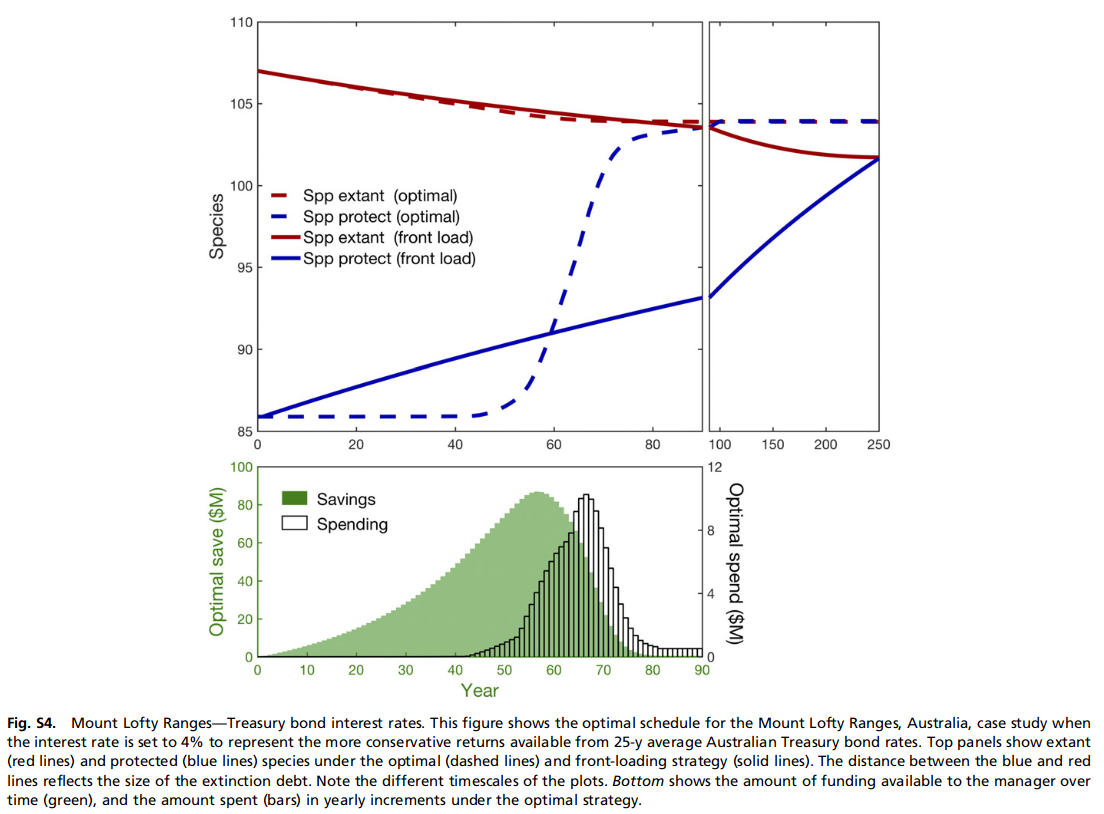
\includegraphics[scale=0.35]{resultsMLR.png}
	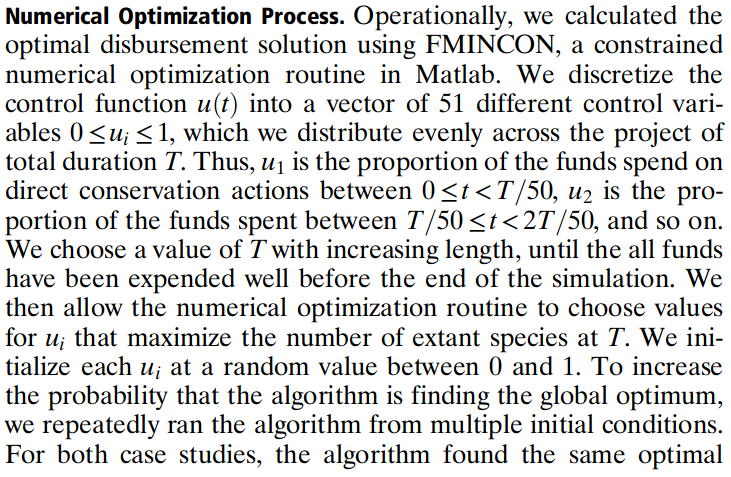
\includegraphics[scale=0.5]{optimisationprocess.png}
\end{center}

\section{Artificial intelligence}

\subsection{Genetic algorithms}

\section{Why do we want to conserve? (From an evolutionary point of view?)}
Caution! Use more conditional mode.\\
Does conservation make sense?
Why do we want it?\\
The scientific/ecological reasons:
\begin{itemize}
    \item Biodiversity is necessary for the maintain of the ecological balance (we depend on).
    \item It fuels evolution.
    \item We strongly depend on environmental services (pollination, CO2 absorption, maintain of soil, bio-degradation, soil maintenance, and many more), that might be affected by losses of biodiversity. 
    \item Biodiversity insure a quick and adapted response to change. Some of which are useful to us (lots of cure molecules were discovered thank to species that already used it).
    \item Source of inspiration through biomimetism.
    \item \dots
\end{itemize}
The ("non-scientific") non-ecology-related reasons:
\begin{itemize}
    \item We like the way nature looks, \textbf{we do not want it to change}, we want it to stay the way we used to know it. Or we know it works kind of fine this way, and letting it change uncontrollably could lead to a less suitable habitat for us.
    \item We want to leave a beautiful world to our offspring, at least as beautiful as ours. \textbf{Beautiful or just suitable?.} Interestingly, this could be interpreted as an evolutionary-driven behaviour; we were successful in that environment, we assume that our descendants are more likely to be as successful in the same environment. The chances are lower if the environment changes too much, or faster than they can adapt to.
    \item It might be a simple intent to indirectly conserve our species, because we rely on a healthy environment.
    \item We like having some species around, because they are cute or directly useful to us.
    \item It gives us an ethical purpose. We feel better trying to act on it, a sort of compensation for us being at the origin of the problem. Would any other species do that?
    \item Could also be a simple scientific curiosity for the topic. Which would be more understandable than any other reason to me.
    \item Being in control of one's environment seems satisfying to us, it is a feel of power.
    \item Having a socially accepted/recognized life goal, because in our society we are mostly defined by our occupation.
    \item Researcher are often further needed to justify their intellectual work, putting "conservation" on it makes consensus on its social "utility".
\end{itemize}

Luc after someone's response at the lab drink: "Is that a satisfactory answer to your question? We conserve because we want to."
From the game-theoretic point of view, most people value (associate a positive utility to) the fact of having access to nature. They also value certain "sexy species".
But most of them also despise some aspects of the biodiversity that goes with it (insects, weed plants), and would rather not have them around (negative utility).

We might also be preventing species from evolving by maintaining their environment in a relatively steady state, thus slowing the adaptation process, getting on "its" way.

Being a pro-conservation has became the norm in "developed" countries, and anyone that would think otherwise might be ostracised.
(Same with feminism, I believe going against it, or not being aware of the problem, will significantly reduce chances to seduce a girl.)
It became a must-have to be part of a "northern modern society".
Being aware of it, seeing it as a concern, is seen as a positive signal by the community.

If it was actually/strictly environmentally-driven, it would be quite paradoxical because we are, very likely, the source of unprecedented perturbations in the ecosystem(s).
Through conservation, we extend our time spent on Earth, and delay our population drop/the natural control of our population. 
(Are we living above our carrying capacity? Probably, because it's a known fact that one planet is not enough to sustain 7 billions people living the northern way of life.)
But does it makes sense for species to embrace its own population control? We could avoid extinction, just by conserving ourselves the way we do with other species.
It is controversial, we don't mind letting farmers shoot geese when managers judge it necessary, but would we let that happen on our own species?
\textbf{Are we legitimate to act on the conservation of any species, knowing that we are not willing to deal with the initial issue which is our life style?}

A typical answer would be "it would be worse if we do nothing", but is that a correct thinking?
The dynamic and complexity of ecosystems are unreachable for our minds, or machines, who knows what could be the actual outcome of such species going extinct.
Extinctions and emergence of new species is a well established cycle, it would be interesting to see at which rate species are disappearing and emerging, and to investigate the link with human activity.
It would also be interesting to see in which group has which rate and if it changed since our "development".
Seems very tough, given that our methods have and are evolving.
Would it make sense in the way that general, overall biodiversity is not the goal of conservation, but biodiversity inside all the different "functional" groups.

Biodiversity, as the net between ecosystems, species and genetic diversities, is the key for environment to respond to change, and subsist. Losses in any kind of theses bio-diversities, or the links between them, will result in a environment much more sensible/weaker to changes. WHY IS THAT SO CONCERNING? It is for us, because it makes our survival less likely in the future! As species that spawn and fray at the same exact location, we assume, in a evolutionary way that the place we are successful in is the best bet we have. Same when it fells weird to leave your home-town to settle elsewhere. We are afraid of change, of uncertainty, because we want to persist in the environment we are successful in? \textbf{Which might cause divergences when someone involved in a conservation process is less successful in his environment, maybe he wants it to change!}\\

7/11/18 Challenge Debate: Do we have a moral responsibility to save the planet?
Tom said that we have limited empathy for what goes beyond our close circle of relationships, which can explain why we care so few about others, or our environment.
\textbf{Do conservationists have a higher empathy ability?}
Holland, in \cite{redpath2015conflicts} second chapter emphasise on the distinction we make between our relatives and our environment.\\
Sam said that there are other problems more important to resolve, like hunger, homelessness, war, \dots. Alistair answered that most of these problems rise from a unequal repartition, and misuse of resources. He believe that these problems are highly interconnected, and that a better management of the environment would participate to the attenuation of these. I think that as he chose a scientific career, it is probably a good thing he can do to involve in the resolution of these problems.

Post on Sti-CS website: What kind of conservationist are you?
Cf futureconservation.org.
A questionnaire supposed to identify which kind between New Conservationist (conservation is about human well-being rather than nature's sake. Emphasise on the role of biodiversity in economic growth. More generally, including nature in the economic system so people care more.), Market Biocentrist (promote free market to let more sustainable markets to develop thus reducing our resources consumption), Critical Social Scientist (see below - Growth and market sceptic, understanding that conservation has to include people's life and well-being), Traditional Conservationist (Mainly nature-driven, with human well-being in mind but not a actual goal, promote protected areas, mainly in yet untransformed landscaped as preventive measures). Some trouble hesitating to answer "aspirationally (this is how it should be) or more realistically (this is how it should be, given the circumstances)". 

My answers to the questions:\\
\textbf{Advancing the well-being of all people should be a goal of conservation.} Disagree - The goal of conservation is to manage our impact on wildlife, by being aware of the consequences of our actions so we can choose them wisely. If it result in better well-being it's great but it is not a goal \textit{per se} to me.\\
\textbf{Non-native species offer little conservation value.} Disagree - The value we attribute species should be adaptive, they now belong to the "previous" ecosystem and are thus part of its balance. They should enter in the scope of conservation as well.\\
\textbf{Conservation goals should be based on science.} Slightly disagree - Conservation should be based on both sciences and empirical knowledge on inhabitants expectations. Sustainable management strategy can only emerge when every party is happy with it.\\
\textbf{Human affection for nature grows in line with income.} Disagree - Sometimes the poorest people rely a lot on what we call "ecological services" for "survival" so they might care a lot for nature. But very rich people tend to not care that much in comparison to fortune. But as soon as something "natural" is an income resource, they might be very focused on it and forget about nature in a broader sense. There might be a difference to make between people using ecological services as source of monetary income and those needing them to survive. Among the first kind, it might be a sort of Gaussian relationship, \textit{might be interesting to check}.\\
\textbf{Protecting nature for its own sake does not work.} Strongly agree - It has to include human interests so it can be efficient and sustainable.\\
\textbf{There is a risk that economic rationales for conservation will displace other motivations for conservation.} Agree - And it could lead to species interesting to humans to get more attention and feed what I would call the "monoculture" effect.\\
\textbf{Conservation messages that emphasise the value of nature for nature's own sake are more effective than those that promote the benefits of nature to humans.} Agree - the masses seem more sensible to the extinction of species than the loss of income of farmers.\\
\textbf{Conservation should work with, not against, capitalism.} Disagree - Capitalism is kind of antinomian to conservation to me, but it can use its semantic/logos to make stakeholders agree on the fact that unlimited exploitation is not a sustainable solution.\\
\textbf{Conserving nature for nature's sake should be a goal of conservation.} Slightly disagree - I like the way nature is right now, would be glad to continue seeing it that way, but it should not be a goal of conservation. It should focus on reducing and avoiding conflict with humans.\\
\textbf{To achieve conservation goals, human population growth must be reduced.} Slightly disagree - It would be a very efficient solution but not doable, what is more feasible is changing northern consumerism.\\
\textbf{Conservation goals should be based on ethical values.} Disagree - Ethics are rooted in culture too much, and differs greatly to one another.\\
\textbf{Strict protected areas are required to achieve most conservation goals.} Neutral - If the area has been specifically dedicated to it, yes. But one could also think of these places as a haven of human non-interference.\\
\textbf{Giving a voice to those affected by conservation actions improves conservation outcomes.} Strongly agree - Involvement is more efficient than enforcement.\\
\textbf{To achieve its goals, conservation should seek to reform global trade.} Disagree - If the exploitation were meant to provide for local populations only, I suspect they would be smaller, and would be less likely to enter in complex conflict with wildlife.\\
\textbf{Economic arguments for conservation are risky because they can lead to unintended negative conservation outcomes.} Slightly agree - Could lead to more "monoculture".\\
\textbf{The best way for conservation to contribute to human well-being is by promoting economic growth.} Strongly disagree - Economic growth is a irrational concept that is absolutely not sustainable, and should not be promoted by anything.\\
\textbf{Conservation must benefit poor people because to do so is an ethical imperative.} Disagree - It does not have to benefit anyone, it has to trade-off.\\
\textbf{Pristine nature, untouched by human influences, does not exist.} Slightly disagree - Even thought you can find plastic shreds pretty much everywhere, I believe there are still places where human influence is anecdotic.
\textbf{Maintaining biological diversity should be a goal of conservation.} Agree - It is a necessary condition for the well-being of an ecosystem.\\
\textbf{There is no significant conservation value in highly modified landscapes.} - Slightly disagree - Even if there is not much left to conserve, highly modified landscapes can still use ecological services, and they can help reducing energy consumption.\\
\textbf{Nature often recovers from even severe perturbations.} Strongly agree - Yet it might be in a very unpredictable way and might never resemble what we knew before, nor being suitable for humans or many other contemporary species.\\
\textbf{Having multiple rationales for conservation weakens the conservation movement.} Disagree - Even if it makes it more complex, it makes it more adapted, adaptive and sustainable.\\
\textbf{Conservation actions should primarily be informed by evidence from biological science.} Agree - But also by any kind of other tangible evidence.\\
\textbf{To achieve conservation goals, the environmental impact of the world's rich must be reduced.} Agree - Them first, but much better if every one could do the same.
\textbf{Working with corporations is not just pragmatic; they can be a positive force for conservation.} Slightly agree - It can be a marketing force, but I would be surprised if it was not productivity driven.\\
\textbf{Humans are separate from nature, not part of it.} Slightly agree - They have means of resources assimilation that put them aside from the rest of the species, but they interact with nature just as much as every other and impact them in a much greater way, so they are still part of it. They just suffer less natural selection \textit{(is there a way to assess the intensity of selection in population genetics?)}.\\
\textbf{Conservation communications are more effective when they use negative 'doom and gloom' messages rather than positive messages.} Slightly agree - people are more sensible to their own threat, or to the suffering of charismatic animals.\\
\textbf{When communities manage their own resources, their efforts are more effective than top-down approaches.} Agree - Involvement is stronger than enforcement.\\
\textbf{Conservation should seek to reduce the emotional separation of people from nature.} Slightly agree - It goes with being conscious of the consequences of its loss, but not necessary. People just has to understand the consequences and agree with the solution.\\
\textbf{Conservation will only be a durable success if it has the support of corporations.} Disagree - No one needs their support, conservation is also about gaining confidence on our individual value and consequences of our actions. \textit{Corporations are deflective shield, we go through them so we don't face the consequences of our consumerism.} Yet, they can help spreading a way of thinking.\\
\textbf{Giving a voice to those affected by conservation action is an ethical imperative.} Slightly disagree - It is just the most efficient way.\\
\textbf{Maintaining ecosystem processes should be a goal of conservation.} Agree - They are the key of balance.\\

\begin{center}
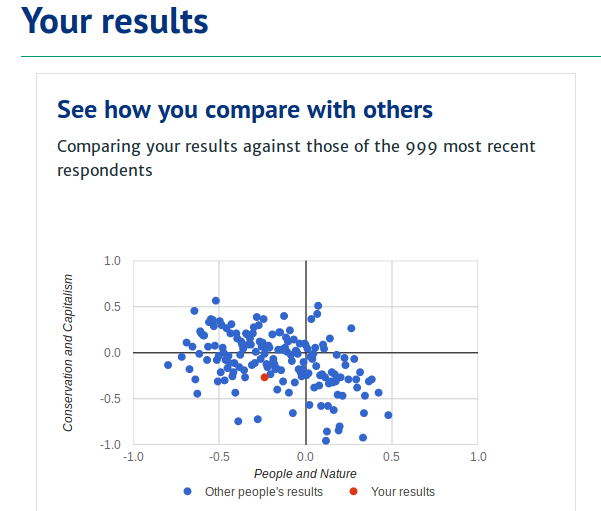
\includegraphics[scale=0.5]{results.png}
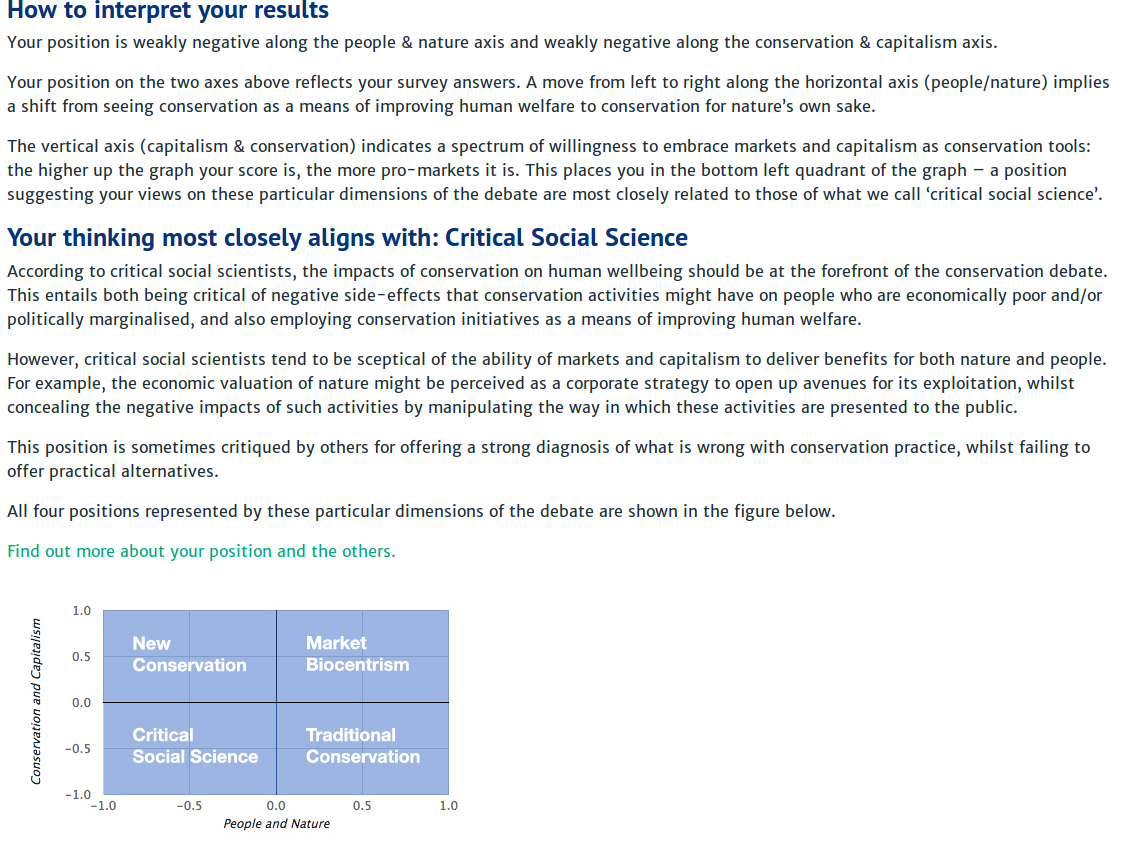
\includegraphics[scale=0.4]{interpretation.png}
\end{center}

\section{AI ethics}
\newpage
\bibliography{PhD-litReview}
\nocite{*}
\end{document}
